% Adjust these for the path of the theme and its graphics, relative to this file
%\usepackage{beamerthemeFalmouthGamesAcademy}
\usepackage{../../beamerthemeFalmouthGamesAcademy}
\usepackage{multimedia}
\graphicspath{ {../../} }

% Default language for code listings
\lstset{language=C++,
        morekeywords={each,in,nullptr}
}

% For strikethrough effect
\usepackage[normalem]{ulem}
\usepackage{wasysym}
\usepackage{graphicx} %package to manage images

\usepackage{pdfpages}

% http://www.texample.net/tikz/examples/state-machine/
\usetikzlibrary{arrows,automata}

\newcommand{\modulecode}{COMP702}\newcommand{\moduletitle}{Classical Artificial Intelligence}\newcommand{\sessionnumber}{1}

\begin{document}
\title{\sessionnumber: Module Introduction}
\subtitle{\modulecode: \moduletitle}

\begin{frame}
	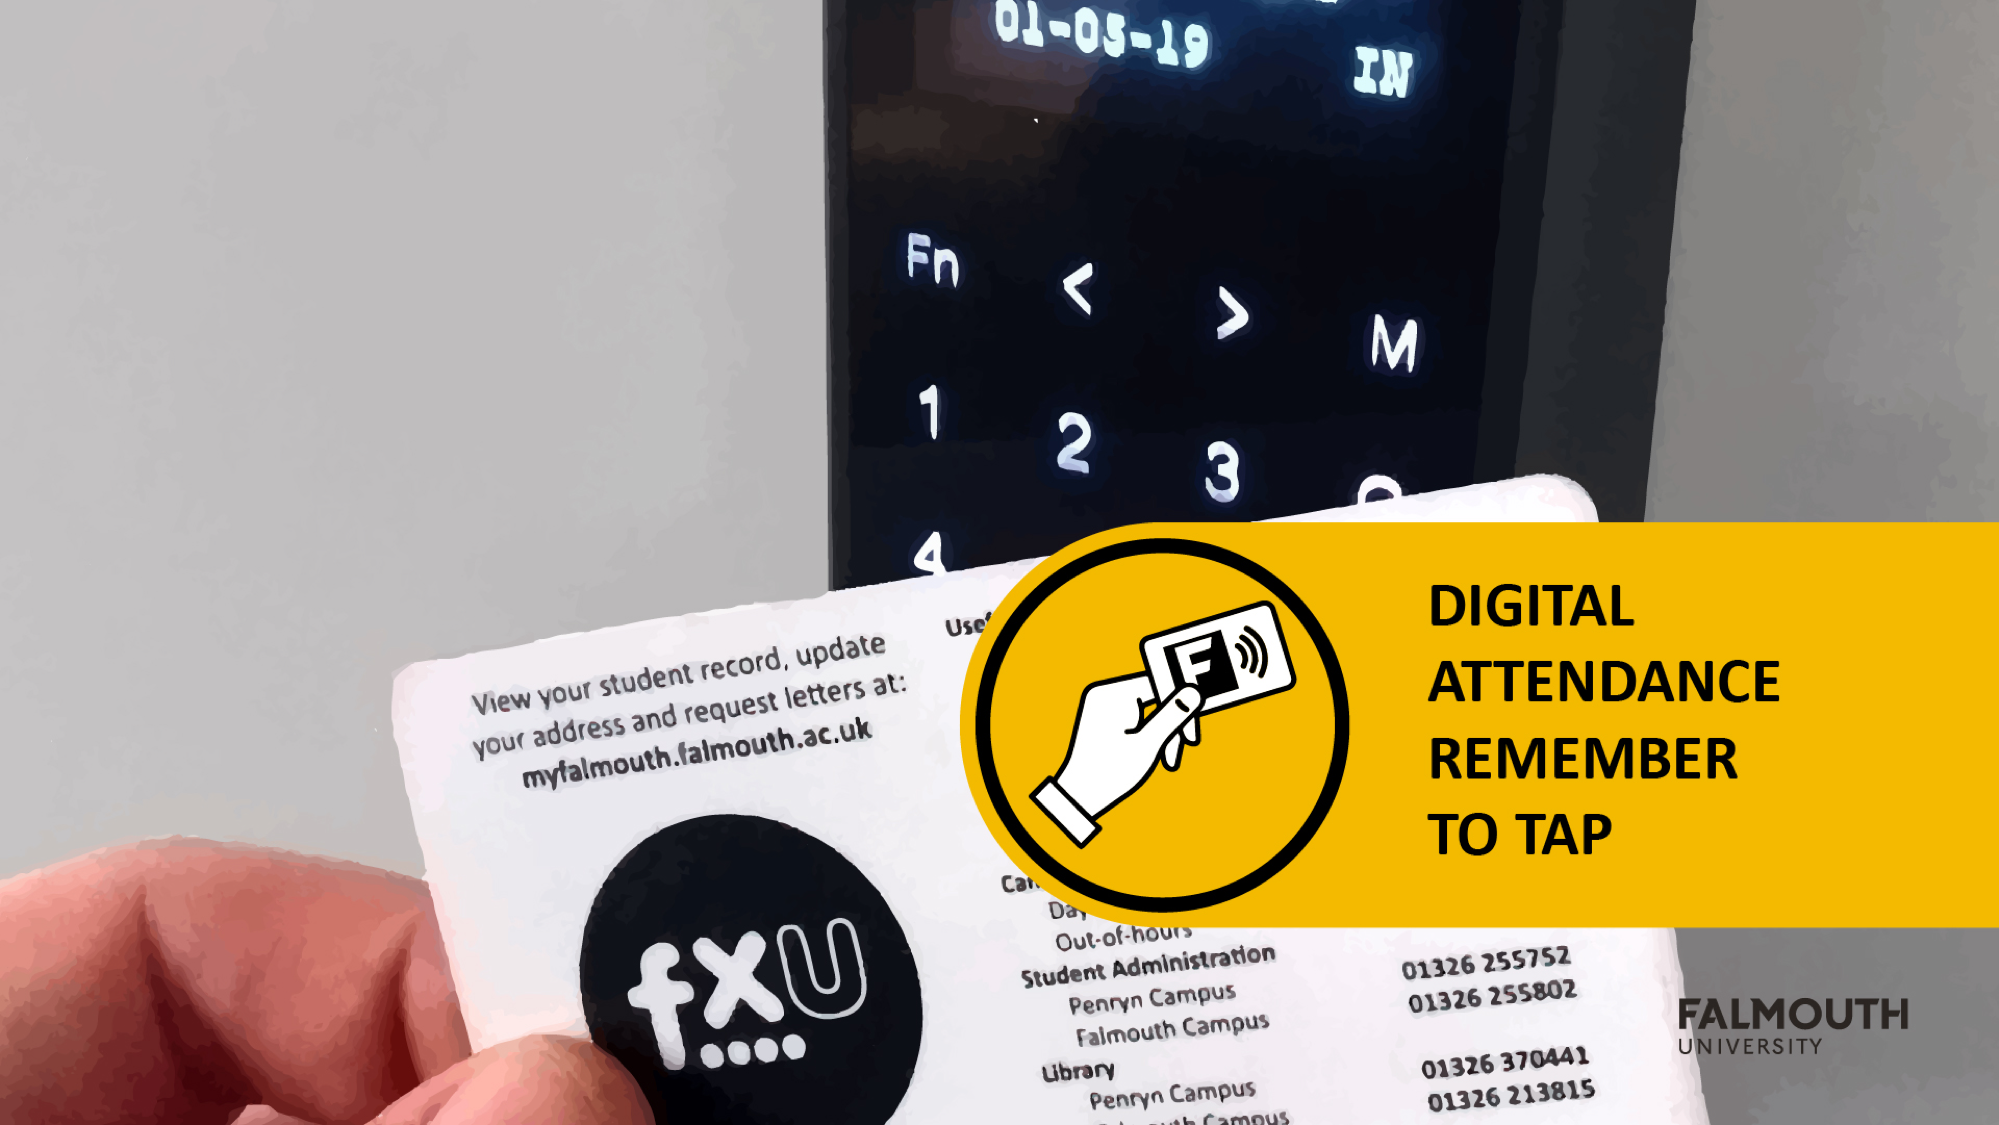
\includegraphics[width=1.0\textwidth]{sign-in}
\end{frame}

\frame{\titlepage} 


\begin{frame}{Today's agenda}
	\begin{itemize}
		\item GAM702 course outline
		\item GAM702 assignment
		\item First brief
	\end{itemize}
\end{frame}

\begin{frame}{First Prototype - DIY}
\begin{center}
	\Huge{Due Friday 5pm on Week 3!}
\end{center}
\end{frame}

\part{Iterative Development}
\frame{\partpage}

\begin{frame}{Iterative Game Design Process}
	\begin{figure}
		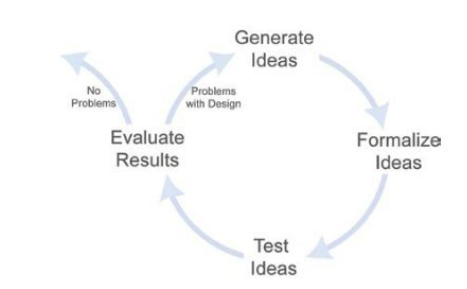
\includegraphics[width=1.0\textwidth,height=0.7\textheight]{iterative_game_design}
		\caption{taken from Game Design Workshop}
		\label{fig:iter1}
	\end{figure}
	\note[item]{Set player experience goals}
\end{frame}

%Set player experience goals
%Brainstorm ideas
%Build a prototype or document system/gameplay etc
%Test ideas (expert or audience)
%Evaluate results
%if idea doesn't work at all, start the process over
%if idea works, modify and test again

\begin{frame}{Design Thinking}
	\begin{figure}
		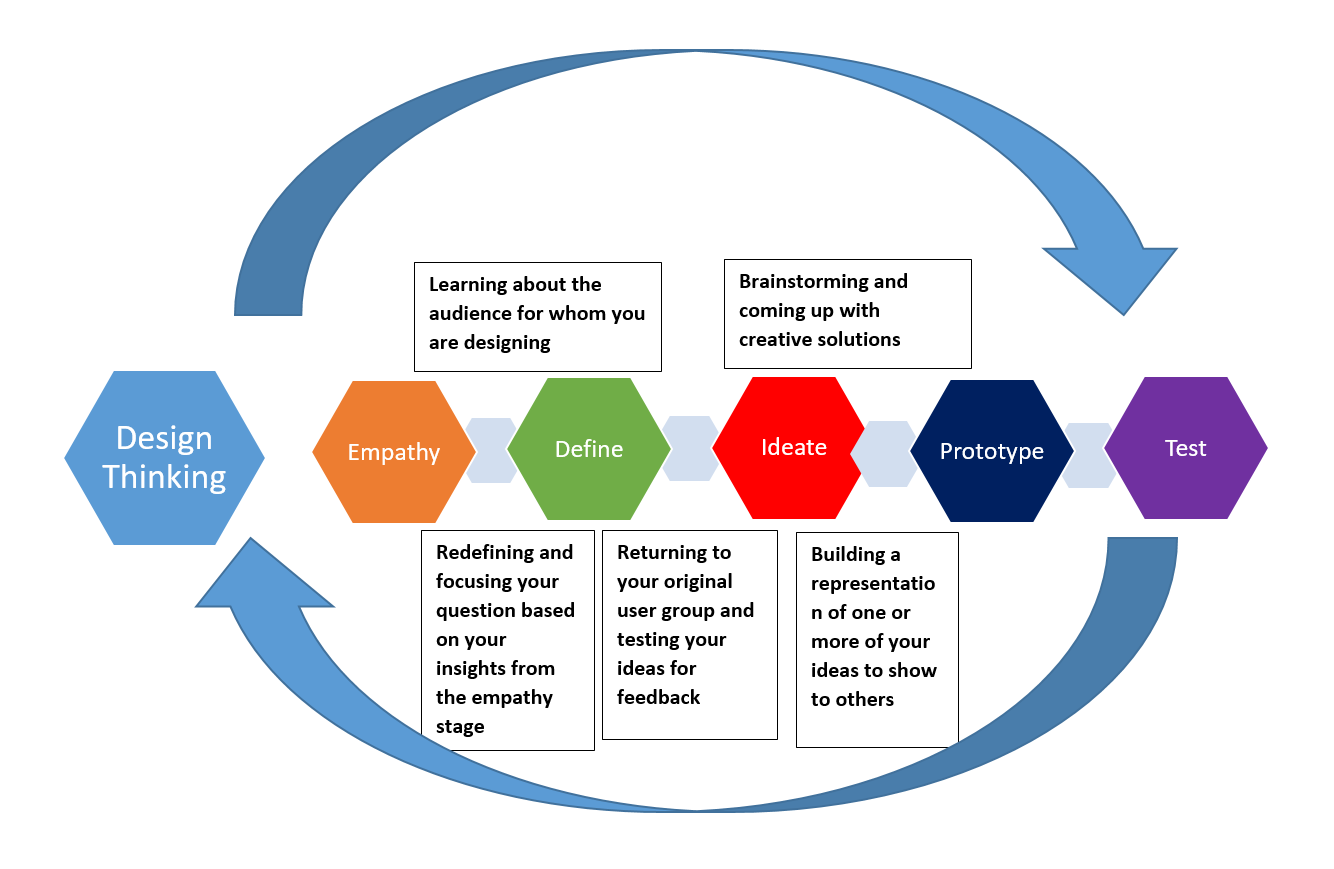
\includegraphics[width=1.0\textwidth, height=0.7\textheight]{design_thinking}
		\label{fig:design_thinking1}
	\end{figure}	
\end{frame}

%important to remember that you can jump around

\begin{frame}{Double Diamond}
	\begin{figure}
		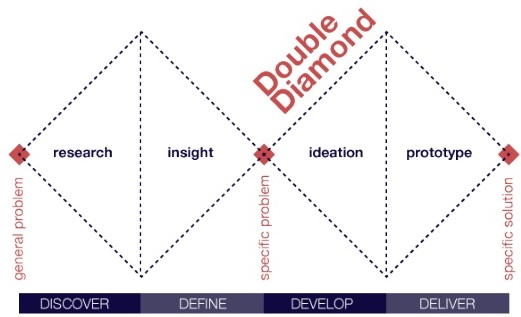
\includegraphics[width=1.0\textwidth, height=0.7\textheight]{double_diamond}
		\label{fig:double_diamond}
	\end{figure}
\end{frame}

%Created by the Design Council
%Discover. The first diamond helps people understand, rather than simply assume, what the problem is. It involves speaking to and spending time with people who are affected by the issues.
%Define. The insight gathered from the discovery phase can help you to define the challenge in a different way.
%Develop. The second diamond encourages people to give different answers to the clearly defined problem, seeking inspiration from elsewhere and co-designing with a range of different people. 
%Deliver. Delivery involves testing out different solutions at small-scale, rejecting those that will not work and improving the ones that will.

\begin{frame}{Summary}
\begin{itemize}
	\item Notice the key similarities in these models
	\item Iteration, testing and revising are key
	\item For the rest of this lecture we are going to focus on the ideation stage
\end{itemize}
\end{frame}
\input{ideaisation}


}
\end{document}
